\documentclass{beamer}
\usepackage[utf8]{inputenc}
\usepackage{amsmath, amssymb, amsthm}
\usepackage{tikz}
\usepackage{listings}
\usepackage{mathtools}


\usetheme{CambridgeUS}
\usecolortheme{crane}

\title{From Abstraction to Computation: \\ Understanding Lambda Calculus}
\author{Pratham Gupta  Gavish Bansal\\
        Sehaj Ganjoo  Krishna Agarwal}
\institute{Indian Institute of Science, Bengaluru}
\date{\today}

\AtBeginSection[]
{
  \begin{frame}[allowframebreaks]
    \frametitle{Outline}
    \tableofcontents[currentsection]
  \end{frame}
}

% \AtBeginSubsection[]
% {
%   \begin{frame}[allowframebreaks]
%     \frametitle{Outline}
%     \tableofcontents[currentsection,currentsubsection]
%   \end{frame}
% }


\begin{document}

% Slide 1: Title Slide
\begin{frame}
  \titlepage
\end{frame}

% Slide 2: Outline
\begin{frame}{Outline}
  \tableofcontents
\end{frame}

% Section 1: Introduction and Motivation
\section{Introduction and Motivation}

\begin{frame}{Historical Background}
\textbf{Leibniz’s Ideal:}
\begin{itemize}
    \item A "universal language" to express all possible problems.
    \item A decision method to solve all problems in this language.
\end{itemize}
\bigskip
By the early 20th century, set theory and first-order logic (Frege, Russell, Zermelo) fulfilled point (1).\\
However, point (2) remained open—this became the Entscheidungsproblem ("decision problem"):\\
\begin{quote}
    Can all problems be solved mechanically?
\end{quote}
\end{frame}
\begin{frame}{Historical Background}
Alonzo Church and Alan Turing independently proved that no general algorithm can decide the truth of all mathematical statements.\\
In order to do so, they had to formalize "computability.\\
\begin{itemize}
    \item Church (1936): Introduced lambda calculus as a formal model of computation
    \item Turing (1936/37): Introduced Turing machines as an alternative model.
    \item Turing (1937): Proved both models are equivalent—defining the same class of computable functions
\end{itemize}

\end{frame}
%Hilbert’s Entscheidungsproblem (1928):
% (“decision problem”)
% Given a sentence in first-order logic, give an “effectively calculable procedure” for determining if it’s provable.
% Mathematicians: “we should probably try to formalize what counts as an ‘algorithm’ ”.
% \begin{frame}{Historical Background}
%   \begin{itemize}
%     \item Developed by Alonzo Church in the 1930s.
%     \item Originally intended as a foundation for mathematics.
%     \item Inspired by higher-order logic and the concept of functions.
%     \item Later became a model of computation equivalent to Turing machines.
%   \end{itemize}
% \end{frame}

\begin{frame}{Motivation}
  \begin{itemize}
    \item Addressing Russell’s paradox in set theory.
    \item Establishing a formal system for computability.
    \item Laying the groundwork for functional programming languages.
  \end{itemize}
\end{frame}

\begin{frame}{Church-Turing Thesis}
Any natural / reasonable notion of computation realizable in the physical world can be simulated by a TM (or equivalently, by lambda calculus)
\end{frame}

\begin{frame}{Overview of Topics}
  \begin{itemize}
    \item Syntax of the lambda-calculus.
    \item Free and bound variables.
    \item Substitution and $\alpha$-conversion.
    \item $\beta$-reduction and the Church–Rosser theorem.
    \item Combinators and representation of booleans.
    \item Encoding natural numbers.
    \item Fixed-point combinators and recursion.
    \item $\lambda$-definability of computable functions.
  \end{itemize}
\end{frame}

% Section 2: Syntax of the Lambda Calculus
\section{Syntax of the Lambda Calculus}
\begin{frame}{Basic Concepts}
  \begin{itemize}
    \item \textbf{Variables:} $x, y, z, \dots$
    \item \textbf{Abstraction:} $\lambda x.M$ (function definition)
    \item \textbf{Application:} $(MN)$ (function application)
  \end{itemize}
\end{frame}

\subsection{$\lambda$-Terms}
\begin{frame}{Formal Definition of $\lambda$-Terms}
  \begin{block}{Definition}
    The set of $\lambda$-terms is defined inductively:
    \begin{enumerate}
      \item Any variable $x$ is a $\lambda$-term.
      \item If $M$ and $N$ are $\lambda$-terms, then $(M N)$ is a $\lambda$-term called an \textbf{application}
      \item If $M$ is a $\lambda$-term and $x$ is a variable, then $\lambda x.M$ is a $\lambda$-term called a $\lambda$-abstraction
    \end{enumerate}
  \end{block}
  % \textbf{Examples:}
  % \begin{itemize}
  %     \item Let \(M = \lambda x.x\), which is a lambda abstraction.
  %     \item Let \(N = y\).
  %     \item \((M N) = (\lambda x.x \; y) \rightarrow y\).
  % \end{itemize}
\end{frame}

\begin{frame}{Formal Definition of $\lambda$-Terms}
  \begin{block}{Some Valid Lambda Expressions:}
  \begin{itemize}
      \item $x$
      \item $\lambda x.x$
      \item $xy$
      \item $x\lambda y.(x(yy))$
      \item $\lambda x.\lambda y.(x)$ (invalid)
  \end{itemize}
  \end{block}
\end{frame}

\begin{frame}{Tree Representation}
    \begin{itemize}
      \item Each $\lambda$-term can be represented as a labeled tree.
      \item Leaves represent variables.
      \item Interior nodes represent applications or abstractions.
    \end{itemize}
    \begin{center}
      % Replace with your own image if desired
        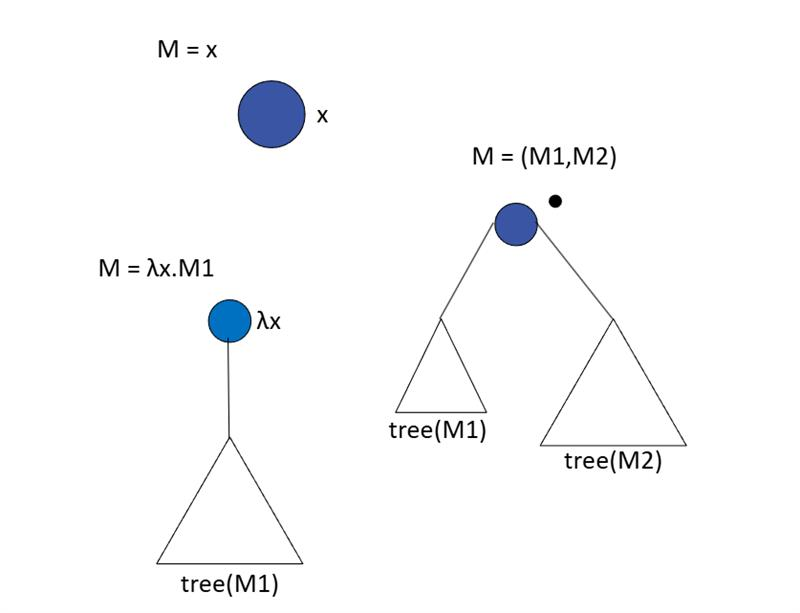
\includegraphics[width=0.5\textwidth]{images/treeimage.png}
    \end{center}
\end{frame}
  


\begin{frame}{Notation Conventions}
  \begin{itemize}
    \item Left-association of application:
      \[
        (((F \; M_1)M_2)\ldots M_n) \quad\text{is written as}\quad F M_1 \ldots M_n.
      \]
      e.g. \(wxyz\) is \(((wx)y)z\).
    \item Right-association of abstractions:
      \[
        \lambda x_1.\lambda x_2.\cdots\lambda x_n.M \quad\text{is written as}\quad \lambda x_1 \cdots x_n.M.
      \]
      e.g. \(\lambda x.xy\) is \(\lambda x.(xy)\), and
      \(\lambda x.\lambda x.x\) is \(\lambda x.(\lambda x.x)\).
  \end{itemize}
\end{frame}
\begin{frame}{Semantics}
  \textbf{$\lambda$x.M} defines a function, where:
  \begin{itemize}
    \item $x$ is the formal parameter of the function.
    \item $M$ is the body of the function.
    \item $M \to M_1 M_2$, function application, similar to calling function $M_1$ and setting its formal parameter to $M_2$.
  \end{itemize}
  \vspace{1em}
  \textbf{Example:}
  \begin{itemize}
    \item $\lambda x.\,+ x 1$ defines a function that adds 1 to its argument.
    \item ($\lambda x.\,+ x 1$) 2 evaluates as $(+ 2 1)$, which is 3.
  \end{itemize}
  \begin{block}{}
    Q. How can + function be defined if abstractions only accept 1 parameter?\\
  \end{block}
\end{frame}
\begin{frame}{Currying}
  Technique to translate the evaluation of a function that takes multiple arguments into a sequence of functions that take a single argument.\\
  \vspace{1em}
  Example:
  \[
  \lambda x.\lambda y.((+ x)y)
  \]
  \[
  (\lambda x.\lambda y.((+ x)y))\ 10\ 20 \rightarrow (\lambda y.((+ 10)y))\ 20 \rightarrow ((+ 10)20) \rightarrow 30
  \]
\end{frame}


\subsection{Free and Bound Variables}
\begin{frame}{Free vs. Bound Variables}

  \begin{definition}
    For any $\lambda$-term \(M\), the \textbf{free variables} (FV) and \textbf{bound variables} (BV) are defined as follows:
    \begin{itemize}
      \item If \(M = x\) is a variable, then:
        \[
        \text{FV}(x) = \{x\}, \quad \text{BV}(x) = \emptyset
        \]
      \item If \(M = (M_1 M_2)\), then:
        \[
        \text{FV}(M) = \text{FV}(M_1) \cup \text{FV}(M_2), \quad \text{BV}(M) = \text{BV}(M_1) \cup \text{BV}(M_2)
        \]
      \item If \(M = \lambda x.M_1\), then:
        \[
        \text{FV}(M) = \text{FV}(M_1) \setminus \{x\}, \quad \text{BV}(M) = \text{BV}(M_1) \cup \{x\}
        \]
    \end{itemize}
  \end{definition}

\end{frame}
\begin{frame}{Free and Bound Variables}
  Examples:
  \begin{itemize}
    \item Is $x$ free in $\lambda x.x$? (No)
    \item Is $x$ free in $(\lambda x.xy)x$? (Yes)\\
    $(\lambda x.xy)x \to (xy)$
  \end{itemize}
  \vspace{1em}
  What is the scope of the variable?\\
  -It is bound by what abstraction?\\
  \begin{itemize}
    \item $(\lambda \textcircled{x}.\lambda y.\textcircled{x}y) (\lambda z.\mathbf{x}z)$
  \end{itemize}
\end{frame}
\begin{frame}{Free and Bound Variables}

  \begin{definition}
    A $\lambda$-term M is closed or a \textbf{Combinator} if it has no free variables, i.e., $\text{FV}(M) = \emptyset$.
  \end{definition}

  Intuitively:
  \begin{itemize}
    \item \textbf{Free Variables (FV):} Occur unbound in a term.
    \item \textbf{Bound Variables (BV):} Declared within a $\lambda$-abstraction.
  \end{itemize}
  \vspace{1em}
  \[
  \text{For } M_1 = \lambda x. (xy), \quad \text{FV}(M_1)=\{y\},\quad \text{BV}(M_1)=\{x\}.
  \]
  \[
  \text{For } M_2 = \lambda x.(\lambda y. (x)), \quad \text{FV}(M_2)=\emptyset,\quad \text{BV}(M_2)=\{x,y\}.
  \]
  Note that:
  \begin{itemize}
    \item \(M_2\) has no free variables and is a combinator.
    \item If we rename a bound variable in a term, It has no effect on the behavior of the term.
  \end{itemize}
\end{frame}



% Section 4: Substitution and Alpha-Conversion
\section{Substitution and $\alpha$-Conversion}
% \begin{frame}{$\alpha$ Equivalence}
%   \begin{block}{\strut}
%   Q. What does it mean for two functions to be equivalent?
%   \end{block}
%   - Is $\lambda x.\mathtt{xy} \equiv \lambda y.\mathtt{yx}$?
%   \begin{itemize}
%     \item $\alpha$-equivalence is when two functions vary only by the names of bound variables.
%     \item $M_1 \equiv_{\alpha} M_2$ if $M_1$ can be obtained from $M_2$ by renaming bound variables.
%   \end{itemize}
% \end{frame}
% \begin{frame}{Renaming ($\alpha$ conversion)}
%   $M\{y/x\}$: Rename bound variable $x$ to $y$ in $M$.\\
%   \vspace{1em}
%   \begin{itemize}
%     \item $x\{y/x\} = y$ and $z\{y/x\} = z$ if $z \neq x$.
%     \item $(M_1 M_2)\{y/x\} = (M_1\{y/x\})(M_2\{y/x\})$
%     \item $(\lambda x.M)\{y/x\} = (\lambda y.M\{y/x\})$
%     \item $(\lambda z.M)\{y/x\} = (\lambda z.M\{y/x\})$ if $x \neq z$.
%   \end{itemize}
% \end{frame}


% \begin{frame}{$\alpha$-Equivalence}
%   Example:\\
%   \[
%   (\lambda x. x \lambda y. xyz) \{w/x\} \longrightarrow
%   (\lambda x. x) \{w/x\} (\lambda y. xyz) \{w/y\} \longrightarrow
%   (\lambda y. y) (\lambda y. wyz)
%   \]
%   \begin{itemize}
%     \item Renaming bound variables to avoid clashes.
%     \item \(\lambda x.M \equiv_\alpha \lambda y.M\{y/x\}\) provided \(y \notin FV(M)\).
%     \item Essential for correct substitution.
%   \end{itemize}
% \end{frame}

\begin{frame}{Substitution}
  Our goal: Reduce expressions by replacing variables with terms.\\
  e.g ($\lambda x.x$) 2 $\to$ 2\\
  \vspace{1em}
  \begin{block}{}
  Solution : Substitution Operation
  \end{block}
  \begin{itemize}
    \item Notation: $M[x \to N]$.
    \item Replacing all free occurrences of a variable $x$ in $M$ by a term $N$.
  \end{itemize}
 % Adjust spacing to avoid overfull box
  Example:
  \begin{itemize}
    \item  $(+x1)[x\to 2]$ = (+2 1)
    \item $(\lambda x.(+x1))[x\to 2]$ = $(\lambda x.(+x1))$ (no free $x$)\\
  \end{itemize}
\end{frame}

\begin{definition}
  A substitution $\varphi = [x_1 := N_1, \ldots, x_n := N_n]$ is a finite set of pairs where each \(x_i\) is a variable and \(N_i\) is a $\lambda$-term.\\
\end{definition}
\begin{definition}
  Given a substitution \(\varphi\) and any variable \(x_i\), \(\varphi_{-x_i}\) is a new substitution obtained by removing the pair \((x_i, N_i)\) from \(\varphi\).\\
\end{definition}


% \begin{frame}{Example of Substitution}
%   \[
%     (\lambda x. (xz)(yz))[y := (vv)] \rightarrow \lambda x.\Bigl(x(λu.v) \Bigr)\Bigl((vv)(λu.v)\Bigr)
%   \]
%   \vspace{0.5em}
%   \begin{itemize}
%     \item Illustrates careful handling to avoid capture.
%   \end{itemize}
% \end{frame}

\begin{frame}{Substitution}
  \frametitle{Substitution Rules}
  
  Given any $\lambda$-term \(M\) and a substitution \(\varphi\), the result of applying \(\varphi\) to \(M\) is denoted by \(M[\varphi]\) and is defined as follows:
  \begin{enumerate}
    \item If \(M\) is a variable \(x\), then:
      \[
      M[\varphi] = 
      \begin{cases} 
        N_i & \text{if } x = x_i \text{ for some } i, \\
        x & \text{otherwise.}
      \end{cases}
      \]
    \item If \(M\) is of the form \((M \; N)\), then:
      \[
      M[\varphi] = (M[\varphi] \; N[\varphi])
      \]
    \item If \(M\) is of the form \(\lambda y.M_1\), then:
      \[
      M[\varphi] = 
      \begin{cases} 
        \lambda y.M_1[\varphi] & \text{if } y \notin \{x_i\}, \\
        \lambda y.M_1[\varphi_{-y}] & \text{if } y = x_i \text{ for some } i.
      \end{cases}
      \]
  \end{enumerate}
\end{frame}

\begin{frame}
  \frametitle{Substitution}

  A \(\lambda\)-term \(M\) is \textbf{safe} for substitution \(\varphi = [x_1 := N_1, \ldots, x_n := N_n]\) if:
  \[
    \text{BV}(M) \cap (\cup_{i=1}^n \text{FV}(N_i)) = \emptyset
  \] 
  that is free variables of \(N_i\) do not become bound in \(M\) after substitution.\\
  \vspace{1em}

  If \(M\) is a combinator, then \(M[\varphi] = M\) for any substitution \(\varphi\).\\

  Some examples of substitution:
  \begin{itemize}
    \item \(y[x:=\lambda x.x] = y\) 
    \item \(y[y:=\lambda x.x] = \lambda x.x\)
  \end{itemize}
\end{frame}


% \begin{frame}
%   \frametitle{Caputuring}

%   Consider:
%   \[
%     \lambda x. (xz)(yz)[y := (xx); z := (\lambda u. v)] = \lambda x. (x(\lambda u. v))((xx)(\lambda u. v))
%   \]

  

% \end{frame}


\begin{frame}{Substitution}
  \begin{block}{Example}
    $(\lambda x.yx)[y \to \lambda z.xz]$
  \end{block}
  \begin{itemize}
    \item Result ? : $(\lambda x.(\lambda z.\textcircled{x}z)x)$
    \item $x \in FV(\lambda z.xz)$
    \item $x \in BV(\lambda \textcircled{x}.(\lambda z.\textcircled{x}z)x)$
  \end{itemize}
  This is called Variable Capture.\\
  \begin{block}{}
    \textbf{Solution:} Use $\alpha$-conversion to rename bound variables before substitution.
  \end{block}
  \vspace{1em}
\end{frame}

% \subsection{$\alpha$-Conversion}
\begin{frame}{Capturing}
  Capturing occurs when a free variable unintentionally becomes bound due to renaming or substitution, altering the meaning of an expression.
  
  \vspace{0.5cm}
  \textbf{Example:}
  \begin{align*}
      & (\lambda x. \lambda y. x) (y) \quad \text{(Original Expression)} \\
      & \text{If we substitute } y \text{ for } x:\\
      & \lambda y. y \quad \text{(Captured! Incorrect meaning)}
  \end{align*}

  \vspace{0.5cm}
  \textbf{Problem:} The free variable \texttt{y} got bound accidentally, changing the function's behavior.
\end{frame}

% Slide 2: Alpha-Conversion
\begin{frame}{$\alpha$-Conversion}
  \textbf{Solution:} Rename bound variables before substitution to avoid conflicts.
  
  \vspace{0.5cm}
  \textbf{Example:}
  \begin{align*}
      & (\lambda x. \lambda y. x) (y) \\
      & \text{Rename } y \text{ to } z \text{ in the inner function:}\\
      & (\lambda x. \lambda z. x) (y) \\
      & \text{Now, substitute } y \text{ for } x:\\
      & \lambda z. y \quad \text{(Correct! Meaning is preserved)}
  \end{align*}

  \vspace{0.5cm}
  \textbf{Conclusion:} Alpha-conversion ensures correct variable scoping by avoiding unintended captures.
\end{frame}

% Slide 1: Definition of Alpha-Conversion
\begin{frame}{Definition of $\alpha$-Conversion}
  \textbf{Immediate Alpha-Conversion} ($\rightarrow_{\alpha}$) allows renaming bound variables in lambda terms while preserving meaning.
  
  \vspace{0.5cm}
  \textbf{Rules:}
  \begin{itemize}
      \item $\lambda x. M \rightarrow_{\alpha} \lambda y. M[x := y]$, if $y \notin FV(M) \cup BV(M)$.
      \item If $M \rightarrow_{\alpha} N$, then $MQ \rightarrow_{\alpha} NQ$ and $PM \rightarrow_{\alpha} PN$.
      \item If $M \rightarrow_{\alpha} N$, then $\lambda x. M \rightarrow_{\alpha} \lambda x. N$.
  \end{itemize}
  
  \vspace{0.5cm}
  \textbf{Alpha-Equivalence:} The reflexive, transitive closure of $\rightarrow_{\alpha}$ is denoted as $\equiv_{\alpha}$, meaning two terms are identical up to renaming.
\end{frame}

% Slide 2: Example of Alpha-Conversion
\begin{frame}{Example: $\alpha$-Conversion}
  \textbf{Stepwise Renaming:}
  \[
      \lambda fx. f(f(x)) \rightarrow_{\alpha} \lambda f. \lambda y. f(f(y)) 
      \rightarrow_{\alpha} \lambda g. \lambda y. g(g(y)) 
      = \lambda gy. g(g(y)).
  \]
  
  \textbf{Explanation:}
  \begin{itemize}
      \item $x$ is renamed to $y$.
      \item $f$ is renamed to $g$.
      \item Meaning is preserved, avoiding variable capture.
  \end{itemize}
\end{frame}

% % Slide 3: Need for Alpha-Conversion Before Substitution
% \begin{frame}{Why Alpha-Conversion Before Substitution?}
%   \textbf{Problem:} Direct substitution can lead to variable capture.
  
%   \vspace{0.5cm}
%   \textbf{Solution:} Rename bound variables in $M$ to avoid conflicts with free variables in $N$.
  
%   \vspace{0.5cm}
%   \textbf{Example:}
%   \begin{align*}
%       (\lambda yz. (xy)z)[x := yz] &\equiv_{\alpha} (\lambda uv. (xu)v)[x := yz] \\
%       &= \lambda uv. ((yz)u)v.
%   \end{align*}
  
%   \textbf{Conclusion:} We must rename bound variables first before substitution to ensure correctness.
% \end{frame}

% Section 5: Beta-Reduction and Church–Rosser
\section{Beta-Reduction and Church–Rosser}
\begin{frame}{Beta-Reduction}
  \begin{block}{Definition}
    The relation \(\rightarrow_\beta\) called immediate $\beta$-reduction is the smallest relation satisying the property for all $\lambda$-terms \(M,N,P,Q\)
    \[
      (\lambda x.M)N \rightarrow_\beta M[x := N] \text{ where M is safe for substitution \([x := N]\).}
    \]
    \[
      \text{if } M \rightarrow_\beta N \text{ then } MQ \rightarrow_\beta NQ \text{ and } PM \rightarrow_\beta PN
    \]
    \[
      \text{if } M \rightarrow_\beta N \text{ then } \lambda x.M \rightarrow_\beta \lambda x.N
    \]
  \end{block}
  \begin{itemize}
    \item Transitive closure of $\rightarrow_\beta$ is denoted as $\rightarrow^+_\beta$.
    \item reflexive and transitive closure of $\rightarrow_\beta$ is denoted as $\rightarrow^*_\beta$.
    \item \textbf{\(\beta\)-conversion} denoted by $\xleftrightarrow{*}$ is smallest equivalence relation such that:
      \[
        \xleftrightarrow{*} = (\rightarrow_\beta \cup \rightarrow_\beta^{-1})
      \]
  \end{itemize}
  

\end{frame}

\begin{frame}{Examples of $\beta$-Reduction}
  \begin{block}{Example}
    \[
      (\lambda x.x) y \rightarrow_\beta (x)[x := y] \rightarrow_\beta y
    \]
    \[
      (\lambda xy.y)uv = (\lambda x.(\lambda y.y)u)v \rightarrow_\beta ((\lambda y.y)[x:=u])v = (\lambda y.y)v \rightarrow_\beta v 
    \]
  \end{block}
  \begin{block}{example}
    Let \(\omega = \lambda x.(xx)\) then
    \[
      \Omega = \omega \omega = (\lambda x.(xx))(\lambda x.(xx)) \rightarrow_\beta (\lambda x.(xx))[x := \lambda x.(xx)] = \omega\omega =\Omega
    \]
    This example shows that \(\beta\)-reduction may be infinite. This is what gives lambda calculus its power.
  \end{block}
\end{frame}

\begin{frame}
  \frametitle{Example of $\beta$-Reduction}

  \begin{block}{Example}
    \(\beta\)-reduction can have growing terms also:
    \[
      (\lambda x.xxx)(\lambda x.xxx) \rightarrow_\beta (\lambda x.xxx)[x := \lambda x.xxx] = (\lambda x.xxx)(\lambda x.xxx)(\lambda x.xxx)
    \]
    \[
      \rightarrow_\beta (\lambda x.xxx)(\lambda x.xxx)(\lambda x.xxx)(\lambda x.xxx)
    \]
    \[
      \rightarrow_\beta (\lambda x.xxx)(\lambda x.xxx)(\lambda x.xxx)(\lambda x.xxx)\cdots
    \]
  \end{block}
\end{frame}

\begin{frame}{Church–Rosser Theorem}
  % \begin{itemize}
  %   \item Confluence: If \( M \) reduces to both \( M_1 \) and \( M_2 \), then there exists \( M_3 \) such that both \( M_1 \) and \( M_2 \) reduce to \( M_3 \).
  %   \item Implies uniqueness (up to $\alpha$-conversion) of normal forms.
  % \end{itemize}

  \begin{theorem}
    The following properties hold for the \(\lambda\)-calculus:
    \begin{itemize}
      \item \textbf{Confluence:} If \( M \rightarrow^*_\beta N_1 \) and \( M \rightarrow^*_\beta N_2 \), then there exists \( N_3 \) such that \( N_1 \rightarrow^*_\beta N_3 \) and \( N_2 \rightarrow^*_\beta N_3 \).
      
      \item \textbf{Church-Rosser Property:}
        for any two $\lambda$-terms \(M\) and \(N\), if \(M \xleftrightarrow{*}_\beta N\), then there exists a $\lambda$-term \(P\) such that:
        \[
          M \rightarrow^{*}_\beta P \quad \text{and} \quad N \rightarrow^{*}_\beta P
        \]
    \end{itemize}
  \end{theorem}
\end{frame}

\begin{frame}{Church–Rosser Theorem: Visual Representation}
  \begin{columns}
    \column{0.5\textwidth}
    \begin{figure}
      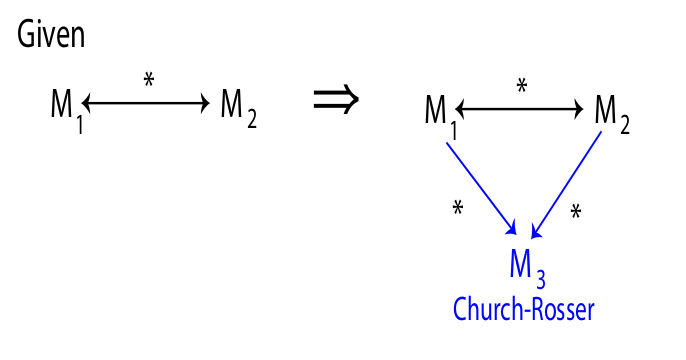
\includegraphics[width=\textwidth]{images/Church-Rosser.png}
      \caption{Church–Rosser Property}
    \end{figure}
    \column{0.5\textwidth}
    \begin{figure}
      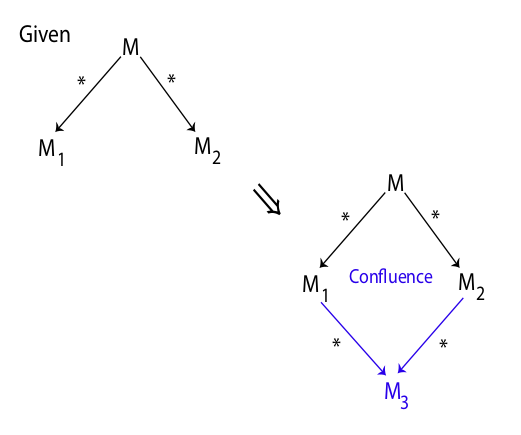
\includegraphics[width=\textwidth]{images/Confluence.png}
      \caption{Confluence Property}
    \end{figure}
  \end{columns}
\end{frame}

% Section 6: Useful Combinators
\section{Some Useful Combinators}

\subsection{Currying}
\begin{frame}
  \frametitle{Currying}
  \begin{block}{Definition}
    In lambda calculus, a abstraction takes only one argument.\\
    \textbf{Currying}( named after Haskell Curry) is the process of transforming a function that takes multiple arguments into a sequence of functions, each taking a single argument.
  \end{block}
  Consider the function: \(f:\mathbb{N}\times\mathbb{N} \rightarrow \mathbb{N}\) \\
  If we fix the first argument, we get a function \(F_x:\mathbb{N} \rightarrow \mathbb{N}\)\\
  \[
    F_x(y) = f(x,y) \forall y \in \mathbb{N}
  \]  
  So we can write \(F_x = \lambda y.f(x,y)\)
  and then the function \(x \mapsto F_x\) can be written as:
  \[
    F = \lambda x.F_x = \lambda x.\lambda y.f(x,y)
  \]
  Hence we obtain 
  \[
    (F\;M)N \rightarrow_\beta F_M N \rightarrow_\beta f(M,N)
  \]
\end{frame}

\begin{frame}
  \frametitle{Currying}

  Hence we have ability to transform a function that takes multiple arguments into a sequence of functions, each taking a single argument.\\
  As a notational convention, we can write:
  \[
  \begin{aligned}
      F &= \lambda x_1.\lambda x_2.\cdots\lambda x_n.f(x_1,x_2,\ldots,x_n) \\ 
        &= \lambda x_1 x_2 \cdots x_n. f(x_1,x_2,\ldots,x_n)
  \end{aligned}
  \]
\end{frame}

\subsection{Bools, Conditional and Pairs}
\begin{frame}{Combinators I, K, and S}
  Let us define the following combinators:
  \begin{itemize}
    \item \( \mathbf{I} = \lambda x.x \) (identity function)
    \item \(\mathbf{T} = \textbf{K} = \lambda xy.x \) (True)

    \item \( \mathbf{F} =\mathbf{K}_* = \lambda xy.y \) (False)
    \item \( \mathbf{S} = \lambda xyz. xz(yz) \) 
  \end{itemize}
  We can see some interesting properties of these combinators:
  \begin{itemize}
    \item \(\mathbf{I}M \rightarrow_\beta M\)
    \item \(\mathbf{K}MN \rightarrow_\beta M\)
    \item \(\mathbf{K}_*MN \rightarrow_\beta N\)
  \end{itemize}
\end{frame}




\begin{frame}{Conditional}
  Let us define the conditional operator:
  \[
    \text{if then else} = \lambda bxy. bxy
  \]
  then for all \(\lambda-terms\) we have:

  \begin{itemize}
    \item \(\text{if}\ \mathbf{T}\ M\ N \rightarrow_\beta M\)
    \item \(\text{if}\ \mathbf{F}\ M\ N \rightarrow_\beta N\)
  \end{itemize}
  Example:
  \[
  \begin{aligned}
      \text{if } \mathbf{T} \text{ then } P \text{ else } Q &= (\text{if then else}) \mathbf{T} P Q \\
      &= (\lambda bxy. bxy) \mathbf{T} P Q \\
      &\rightarrow_{\beta} ((\lambda xy. bxy)[b := \mathbf{T}]) P Q = (\lambda xy. \mathbf{T}xy) P Q \\
      &\rightarrow_{\beta} ((\lambda y. \mathbf{T}xy)[x := P]) Q = (\lambda y. \mathbf{T}Py) Q \\
      &\rightarrow_{\beta} (\mathbf{T}Py)[y := Q] = \mathbf{T} P Q \\
      &= \mathbf{K} P Q \xrightarrow{+}_{\beta} P,
  \end{aligned}
  \]
\end{frame}



\begin{frame}
  \frametitle{Boolean Operations}
  \begin{itemize}
    \item \textbf{And:} \(\text{And }b_1b_2 = \text{if }b_1 \text{ then (if }b_2 \text{ then \textbf{T} else \textbf{F}) else \textbf{F}}\)
    \item \textbf{Or:  } \(\text{Or }b_1b_2 = \text{if }b_1 \text{ then \textbf{T} else (if }b_2 \text{ then \textbf{T} else \textbf{F})}\)
    \item \textbf{Not:} \(\text{Not }b = \text{if }b \text{ then \textbf{F} else \textbf{T}}\)
  \end{itemize}
\end{frame}


\begin{frame}{Constructing Ordered Pairs}
  For any two \( \lambda \)-terms \( M \) and \( N \), consider the combinators \( \pi_1 \) and \( \pi_2 \) defined as:
  \begin{align*}
    \langle M, N \rangle &= \lambda z.\, z\, M\, N \\
    &= \lambda z.\, \text{if } z \text{ then } M \text{ else } N \\
    \pi_1 &= \lambda z.\, zK \\
    \pi_2 &= \lambda z.\, zK_*
  \end{align*}
  Then, we have the following \(\beta\)-reductions:
  \begin{align*}
    \pi_1 \langle M, N \rangle &\xrightarrow{\beta} M \\
    \pi_2 \langle M, N \rangle &\xrightarrow{\beta} N \\
    \langle M, N \rangle T &\xrightarrow{\beta} M \\
    \langle M, N \rangle F &\xrightarrow{\beta} N
  \end{align*}
\end{frame}
\begin{frame}{Proof}
  \begin{block}{Beta Reduction of \(\pi_1 \langle M, N \rangle\)}
    \[
      \pi_1 \langle M, N \rangle \xrightarrow{\beta} M
    \]
  \end{block}
  Proof:  
  We have:
  \begin{align*}
    \pi_1 \langle M, N \rangle &= (\lambda z.\, zK)(\lambda z.\, z M N) \\
    &\xrightarrow{\beta} (zK)[z := \lambda z.\, z M N] \\
    &= (\lambda z.\, z M N)K \\
    &\xrightarrow{\beta} (z M N)[z := K] \\
    &= K M N \xrightarrow{\beta} M
  \end{align*}
\end{frame}
\begin{frame}{Proof}
  \begin{block}{Beta Reduction of \(\pi_2 \langle M, N \rangle\)}
    \[
      \pi_2 \langle M, N \rangle \xrightarrow{\beta} N
    \]
  \end{block}
  Proof:  
  We have:
  \begin{align*}
    \pi_2 \langle M, N \rangle &= (\lambda z.\, zK_*)(\lambda z.\, z M N) \\
    &\xrightarrow{\beta} (zK_*)[z := \lambda z.\, z M N] \\
    &= (\lambda z.\, z M N)K_* \\
    &\xrightarrow{\beta} (z M N)[z := K_*] \\
    &= K_* M N \xrightarrow{\beta} N
  \end{align*}
\end{frame}
\begin{frame}{Proof}
  \begin{block}{Beta Reductions of Ordered Pair Application}
    \[
      \langle M, N \rangle T \xrightarrow{\beta} M, \quad \langle M, N \rangle F \xrightarrow{\beta} N
    \]
  \end{block}
  Proof:  
  We have:
  \begin{align*}
    \langle M, N \rangle T &= (\lambda z.\, z M N) T \\
    &\xrightarrow{\beta} T M N \\
    &\xrightarrow{\beta} M, \quad \text{(since } T = K \text{)} \\[10pt]
    \langle M, N \rangle F &= (\lambda z.\, z M N) F \\
    &\xrightarrow{\beta} F M N \\
    &\xrightarrow{\beta} N, \quad \text{(since } F = K_* \text{)}
  \end{align*}
\end{frame}

% Section 7: Representing Natural Numbers
\section{Representing Natural Numbers}
\begin{frame}{Church Numerals}
  \begin{block}{Definition}
    Church Numerals \(\mathbf{c_0,c_1,c_2,\dots}\) are defined by: 
    \[
      \mathbf{c_n} = \lambda fx. f^n x
    \] 
  \end{block}
  Observe:
  \begin{itemize}
    \item \(\mathbf{c_0} = \lambda fx. x = \mathbf{K_*}\)
    \item \(\mathbf{c_1} = \lambda fx. f x\)
    \item \(\mathbf{c_n} Fz = (\mathbf{c_n}F)z = ((\lambda fx.f^n(x))F)z \rightarrow_\beta^+ F^n(z)\)
  \end{itemize}
\end{frame}

\begin{frame}{Iteration}

  \begin{definition}
    The \textbf{Iteration} combinator \textbf{Iter} is defined as:
    \[
      \text{Iter} = \lambda n f x. n f x
    \]
  \end{definition}
  Notice that:
  \begin{itemize}
    \item Iter combinator is same as the if then else combinator. This means that if we pass a boolean to the Iter combinator then it will behave like the if then else combinator.
    \item \(\text{\textbf{Iter }} \mathbf{c_n} f x = \lambda fx. f^n x\) \\
    proof:
    \[
      \text{\textbf{Iter} } \mathbf{c_n} f x \rightarrow \mathbf{c_n} f x = (\lambda fx.f^n x)fx = f^n x
    \]

  \end{itemize}
\end{frame}

\begin{frame}{Arithmetic Operations}
  \begin{itemize}
    \item \textbf{Successor:} 
    \(\text{\textbf{Succ}}_\text{\textbf{c}} = \lambda nfx.f(nfx)\)
    \item \textbf{IsZero:} 
    \(\text{\textbf{IsZero}}_\text{\textbf{c}} = \lambda x. x(\mathbf{K}\mathbf{F})\mathbf{T}\)
    \item \textbf{Addition:}
    \(\text{\textbf{Add}} = \lambda mn.\text{\textbf{Iter }} m \text{\textbf{ Succ}}_\text{\textbf{c }}n \)
    \item \textbf{Multiplication:}
    \(\text{\textbf{Mult}} = \lambda mn.\text{\textbf{Iter }} m \text{\textbf{ Add}}_\text{\textbf{c }}n\)
    \item \textbf{Exponentiation:}
    \(\text{\textbf{Exp}} = \lambda mn.\text{\textbf{Iter }} n \text{\textbf{ Mult}}_\text{\textbf{c }}m\)
  \end{itemize}
\end{frame}

\begin{frame}{The Predecessor Function}
  \begin{align*}
    \text{Pred}(0) &= 0, \\
    \text{Pred}(n + 1) &= n.
  \end{align*}
  \begin{itemize}
    \item More challenging to define.
    \item Kleene\'s solution in his famous 1936 paper, uses pairs:
    \[
      \text{Pred}_K = \lambda n. \pi_2 (\text{Iter} \ n \ \lambda z. \langle \text{Succ}(\pi_1 z), \pi_1 z \rangle \ \langle c_0, c_0 \rangle).
    \]
  \end{itemize}
\end{frame}
\begin{frame}{The Predecessor Function}
  \textbf{Why Kleene's Predecessor Function Works?}\\
  We have:
  \begin{align*}
    (\lambda z. \langle \text{Succ}(\pi_1 z), \pi_1 z \rangle)^0 \langle c_0, c_0 \rangle &\xrightarrow{\beta} \langle c_0, c_0 \rangle.
  \end{align*}
\begin{block}{We claim that:}
  \begin{align*}
    (\lambda z. \langle \text{Succ}(\pi_1 z), \pi_1 z \rangle)^{n+1} \langle c_0, c_0 \rangle &\xrightarrow{\beta} \langle c_{n+1}, c_n \rangle.
  \end{align*}
\end{block}
\end{frame}
\begin{frame}{The Predecessor Function}
    \begin{align*}Claim:
      (\lambda z. \langle \text{Succ}(\pi_1 z), \pi_1 z \rangle)^{n+1} \langle c_0, c_0 \rangle &\xrightarrow{\beta} \langle c_{n+1}, c_n \rangle.
    \end{align*}
  Proof by Induction on n:\\
  \textbf{Base Case:} \(n = 0\)\\
  \begin{align*}
    (\lambda z. \langle \text{Succ}(\pi_1 z), \pi_1 z \rangle) \langle c_0, c_0 \rangle &\xrightarrow{\beta} \langle \text{Succ}(\pi_1 \langle c_0, c_0 \rangle), \pi_1 \langle c_0, c_0 \rangle \rangle \\
    &\xrightarrow{\beta} \langle \text{Succ}(c_0), c_0 \rangle \\
    &\xrightarrow{\beta} \langle c_1, c_0 \rangle.
  \end{align*}
\end{frame}

\begin{frame}{The Predecessor Function}
  \begin{align*}Claim:
    (\lambda z. \langle \text{Succ}(\pi_1 z), \pi_1 z \rangle)^{n+1} \langle c_0, c_0 \rangle &\xrightarrow{\beta} \langle c_{n+1}, c_n \rangle.
  \end{align*}
  \textbf{Inductive Step:} Assume true for \(n\), show for \(n+1\)\\
  \[
  \begin{aligned}
    &(\lambda z. \langle \text{Succ}(\pi_1 z), \pi_1 z \rangle)^{n+2} \langle c_0, c_0 \rangle \\
    &= (\lambda z. \langle \text{Succ}(\pi_1 z), \pi_1 z \rangle)((\lambda z. \langle \text{Succ}(\pi_1 z), \pi_1 z \rangle)^{n+1} \langle c_0, c_0 \rangle) \\
    &\xrightarrow{\beta} (\lambda z. \langle \text{Succ}(\pi_1 z), \pi_1 z \rangle) \langle c_{n+1}, c_n \rangle \\
    &\xrightarrow{\beta} \langle c_{n+2}, c_{n+1} \rangle.
  \end{aligned}
  \]
\end{frame}
\begin{frame}{Predecessor Functions}
  \begin{itemize}
    \item \textbf{Kleene's predecessor function:}
      \[
      \text{Pred}_K = \lambda n. \pi_2 (\text{Iter} \ n \ \lambda z. \langle \text{Succ}(\pi_1 z), \pi_1 z \rangle \ \langle c_0, c_0 \rangle).
      \]
  
    \item \textbf{Alternative definition of predecessor:}
      \[
      \text{Pred}_c = \lambda x y z.\ x(\lambda p q.\ q(p y)) (K z) I.
      \]
  \end{itemize}
\end{frame}
\begin{frame}{Barendregt Numerals}
  \begin{itemize}
    
    \item Alternative representation: 
      \[
      b_0 = I,\quad b_{n+1} = \langle F, b_n \rangle
      \]
    \item Simpler for certain arithmetic operations.
  \end{itemize}
\end{frame}

% Section 8: Fixed-Point Combinators and Recursion
\section{Fixed-Point Combinators and Recursion}
\begin{frame}{Fixed-Point Combinators}
  \begin{itemize}
    \item Enable recursive definitions without explicit recursion.
    \item \textbf{Curry's Y-combinator:}
      \[
      Y = \lambda f. (\lambda x. f (x x)) (\lambda x. f (x x))
      \]
  \end{itemize}
\end{frame}

\begin{frame}{Properties of the Y-Combinator}
  \begin{itemize}
    \item For any \(F\), \(F (Y F) \equiv_\beta Y F\).
    \item Note: Reduction may not go both ways directly.
  \end{itemize}
\end{frame}

\begin{frame}{Turing's $\Theta$-Combinator}
  \begin{itemize}
  \item Defining the \textit{Turing $\mathbf{\Theta}$-combinator}:
  \[ \mathbf{\Theta} := \left( \lambda xy.y\left( xxy \right)\right) \left( \lambda xy.y\left( xxy \right) \right) \]
  \item Now, for any $\lambda$-term \(F\), we have:
    \[
      \mathbf{\Theta}F \xrightarrow[]{\text{+}}_\beta F(\mathbf{\Theta}F)
    \]
    \textit{Proof:} Writing \( A = (\lambda xy.y(xxy))\). Thus,
    \( \mathbf{\Theta} = AA \). Now,
    \begin{align*}
      \mathbf{\Theta}F &= AA F = ((\lambda xy.y(xxy))A)F\\
      &\xrightarrow[]{}_\beta (\lambda y.y(AAy))F \\
      &\xrightarrow[]{\text{+}}_\beta F(AAF)\\
      &= F(\mathbf{\Theta}F)\\
      & \hspace{5cm} \blacksquare
    \end{align*}
  \end{itemize}
\end{frame}

\begin{frame}{Defining Recursive Functions}
  \begin{itemize}
    \item To define a recursive function \(G\) such that
      \[
      G X \rightarrow_\beta M(X, G)
      \]
    \item Let \(F = \lambda g x. M(x, g)\) and define \(G = \Theta F\).
  \end{itemize}
\end{frame}

\begin{frame}{Example: Factorial Function}
  \begin{itemize}
    \item Define:
      \[
      F = \lambda g\ n.\, \text{if}\ (\text{IsZero}\ n)\ \text{then}\ c_1\ \text{else}\ \text{Mult}\ n\ \bigl(g\ (\text{Pred}\ n)\bigr)
      \]
    \item Then \(G = \Theta F\) represents the factorial function.
  \end{itemize}
  \vspace{-0.5em} % Adjust spacing to avoid overfull box
\end{frame}

% Section 9: Lambda-Definability of Computable Functions
\section{Lambda-Definability of Computable Functions}
\begin{frame}{Computable Functions}
  \begin{itemize}
    \item A function \(f : \mathbb{N}^n \rightarrow \mathbb{N}\) is computable if it can be built from base functions by composition, primitive recursion, and minimization.
  \end{itemize}
\end{frame}

\begin{frame}{Lambda-Definability}
  \begin{itemize}
    \item A function \(f\) is \(\lambda\)-definable if there exists a closed \(\lambda\)-term \(F\) such that:
      \begin{enumerate}
        \item \(F\,c_{m_1}\cdots c_{m_n}\) has a normal form if and only if \(f(m_1,\dots,m_n)\) is defined.
        \item When defined, \(F\,c_{m_1}\cdots c_{m_n} \rightarrow_\beta c_{f(m_1,\dots,m_n)}\).
      \end{enumerate}
  \end{itemize}
\end{frame}

\begin{frame}{Theorem Overview}
  \begin{itemize}
    \item Every total computable function is \(\lambda\)-definable.
    \item Every partial computable function is also \(\lambda\)-definable.
    \item This establishes the equivalence between the lambda-calculus and Turing machines.
  \end{itemize}
\end{frame}

\begin{frame}{Proof Sketch (1): Base Functions and Composition}
  \begin{itemize}
    \item Base functions: zero, successor, and projections are \(\lambda\)-definable.
    \item Closure under composition is straightforward.
  \end{itemize}
\end{frame}

\begin{frame}{Proof Sketch (2): Primitive Recursion}
  \begin{itemize}
    \item Use the iterator combinator and pairing.
    \item Construct a term that computes the recursive function by induction.
  \end{itemize}
\end{frame}

\begin{frame}{Proof Sketch (3): Minimization}
  \begin{itemize}
    \item Define a combinator that searches for the least number \(n\) such that \(g(n,\dots)=0\).
    \item Utilize a fixed-point combinator for the iterative search.
  \end{itemize}
\end{frame}

% Section 10: Summary and Conclusions
\section{Summary and Conclusions}
\begin{frame}{Summary}
  \begin{itemize}
    \item The lambda-calculus provides a minimalistic foundation for computation.
    \item Its syntax is based on variables, abstraction, and application.
    \item Substitution and $\alpha$-conversion manage variable binding.
    \item $\beta$-reduction drives computation.
    \item Combinators, Church numerals, and fixed-point combinators illustrate its power.
    \item Every computable function is $\lambda$-definable.
  \end{itemize}
\end{frame}

\begin{frame}{Implications}
  \begin{itemize}
    \item Equivalence to Turing machines shows universal computation.
    \item Fundamental for the design of functional programming languages.
    \item Offers insights into recursion and fixed-point theory.
  \end{itemize}
\end{frame}

\begin{frame}{Further Directions}
  \begin{itemize}
    \item Study evaluation strategies (call-by-name, call-by-value).
    \item Explore type systems: Simply typed lambda-calculus.
    \item Look into extensions: System F, lambda calculus with recursion.
  \end{itemize}
\end{frame}

\begin{frame}{References}
  \begin{itemize}
    \item Barendregt, H. (1984). \textit{The Lambda Calculus: Its Syntax and Semantics.}
    \item Church, A. (1932-1936). Papers on the lambda-calculus.
    \item Kleene, S. C. (1936). On the normal form theorem.
  \end{itemize}
\end{frame}

\begin{frame}{Acknowledgements}
  \begin{itemize}
    \item Based on a detailed exposition of the lambda-calculus.
    \item Many thanks to the pioneers of lambda-calculus.
  \end{itemize}
\end{frame}

\begin{frame}{Questions?}
  \begin{center}
    \Large Thank you for your attention!\\[1em]
    Any Questions?
  \end{center}
\end{frame}

% Additional slides can be added to reach the 50-60 slide target by expanding on proofs, examples, and further details.

\end{document}
